\PassOptionsToPackage{hyphens}{url}
\documentclass[compress,aspectratio=169]{beamer}

\usetheme{Reading}

\graphicspath{{../2019-06-isc/}{../2019-06-isc/fig/}{img/}{../logo/}}

\newcommand{\ok}[1]{{#1 (done)}}
\newcommand{\ongoing}[1]{{#1 (ongoing)}}
\newcommand{\started}[1]{{#1 (started)}}
\newcommand{\pending}[1]{{#1 (pending in plan)}}
\newcommand{\hrefb}[2]{\href{#1}{\textcolor{blue}{#2}}}

\subtitle{}
\title{\Large Open HPC Certification and Relationship to OSS}
\author{Julian Kunkel (+ HPC Certification Forum)}
\date{2020-11-19}
\authorURL{https://hpc-certification.org}
\authorFooter{Julian M. Kunkel et al.}
\venue{Archer Seminar}
\institute{Department of Computer Science}
\groupLogo{
\includegraphics[width=2.5cm]{hpccf-small}}
\titleLogo{ 
\includegraphics[height=2.5cm]{blur-book-stack-books-590493}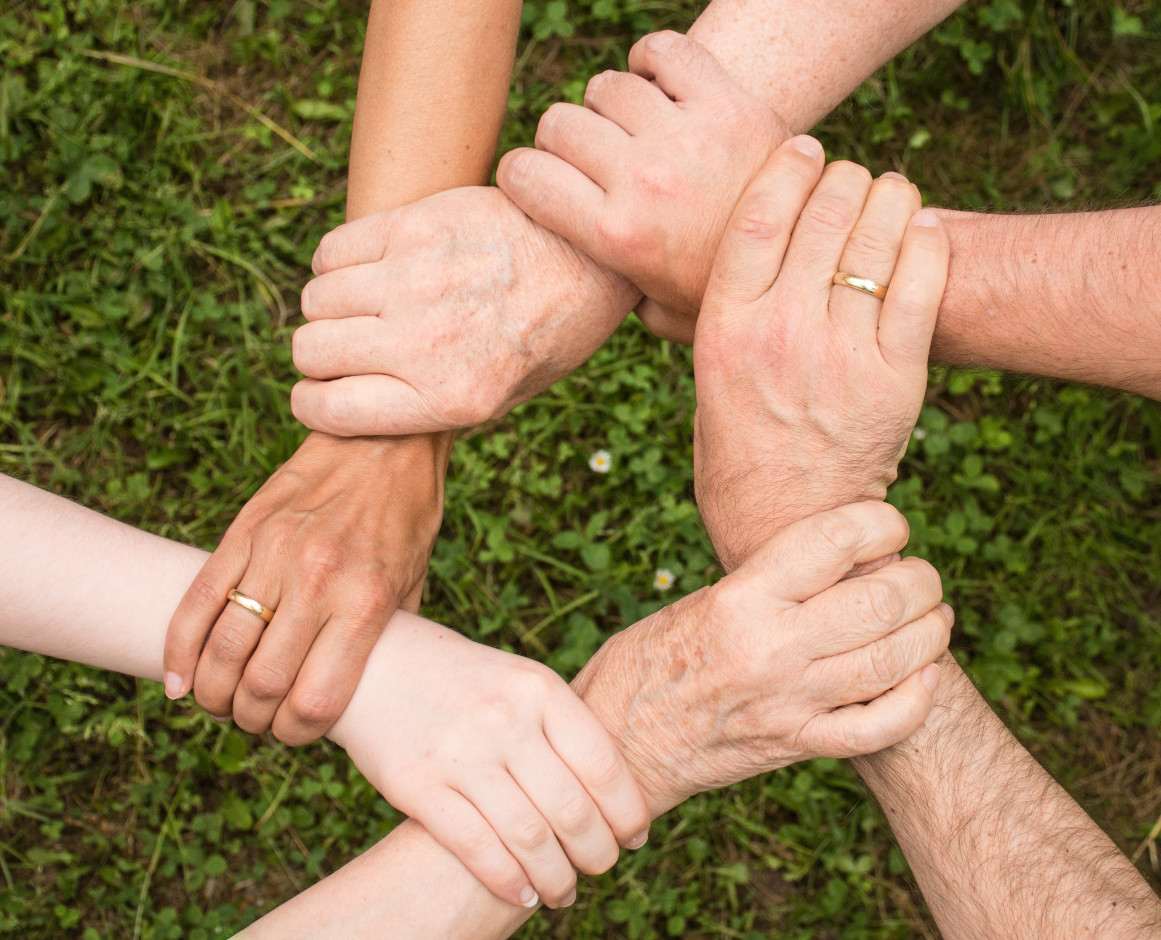
\includegraphics[height=2.5cm]{ground-group-growth-461049}
\includegraphics[height=2.5cm]{accomplishment-ceremony-college-267885}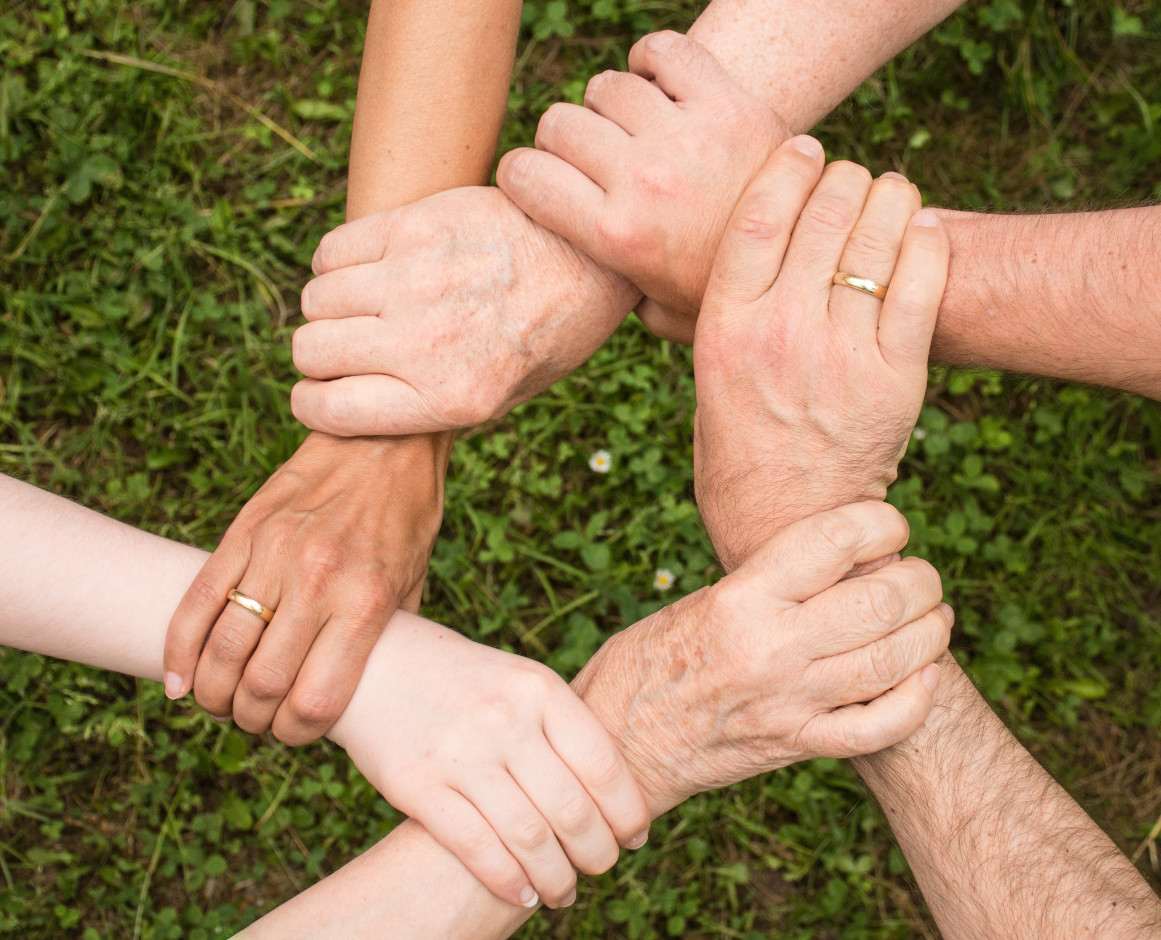
\includegraphics[height=2.5cm]{ground-group-growth-461049}
\includegraphics[height=2.5cm]{blur-book-stack-books-2}}


\begin{document}

\begin{frame}[plain]{}
	\maketitle
\end{frame}


%       the nature of the training or education program
%       Strategy
%       assessment or evaluation technique
%       situations for which it is relevant or in which it was applied
%       an evaluation of its success
%       lessons learned
%       reproducibility of the processes and resources

\section{The Forum}
\sectionIntroHidden

\subsection{}


\begin{frame}{Challenges for HPC Training}
		\begin{itemize}
			\item Not all users possess the right level of training
				\begin{itemize}
				\item Inefficient usage of systems, frustration, lost potential
				\item Good training saves compute time and costs!
				\end{itemize}
      \item Diverse user background and goals
        \begin{itemize}
          \item Science is the goal, HPC is the vehicle
          \item Need to run an application to complete the PhD
        \end{itemize}
      \item Learning is not easy
			\begin{itemize}
				\item Users need to understand beneficial knowledge for tasks
				\item There exist various different training material
				\item Teaching of different data centers is hard to compare
			\end{itemize}
			\item Data center have difficulties to verify the skills of users
		\end{itemize}

\end{frame}


\begin{frame}{The 
\includegraphics[width=0.45\textwidth]{hpccf-full}}
		\begin{block}{Goals}
			\begin{itemize}
				\item Fine-grained standardizing HPC knowledge representation
          \begin{itemize}
            \item What competences exist, how are they defined?
            \item Puzzle of competences for everyone (practitioners, students, admins)
            \item Supporting navigation and role-specific knowledge maps
          \end{itemize}
				\item Establishing international certificates attesting knowledge
        \item Supporting an ecosystem around the HPC competences
			\end{itemize}
		\end{block}

    \begin{block}{Scope of the forum}
    \begin{itemize}
      \item Central authority for competence representation, certification, and support
      \item Purposeful limitations of the forum:
			\begin{itemize}
				\item We do not compete with content providers
				\item We do not create a curriculum (university/centers responsibility)
			\end{itemize}
    \end{itemize}
		\end{block}
\end{frame}


\begin{frame}{The 
\includegraphics[width=0.45\textwidth]{hpccf-full}}

	\begin{block}{Organization Details}
		\begin{itemize}
			\item An independent international body
			\item Organized into
				\begin{itemize}
					\item Steering board (elected)
					\item Full members (with voting rights)
            \begin{itemize}
              \item Contributors to the project (e.g., 1-2 hours per month)
            \end{itemize}
					\item Associate members (anyone and any institution)
          \item Collaboration with e.g., SIGHPC Education Chapter
				\end{itemize}
		\end{itemize}
	\end{block}

	\begin{block}{Responsibilities}
		\begin{itemize}
			\item Curating and maintaining the \textbf{Competence Standard}
			\item Providing tools and ecosystem around the competences
		\end{itemize}
	\end{block}
\end{frame}





\begin{frame}{Governance}
	\smallskip
  We have governance rules splitting responsibility across roles
  \begin{block}{Steering Board}
  \vspace*{-0.5em}
  \begin{itemize}
    \item General chair: Julian Kunkel (University of Reading)
    \item Skill-tree curator: Kai Himstedt (University of Hamburg)
    \item Topic curators:
    \begin{itemize}
      \item HPC Knowledge: Lev Lafayette (University of Melbourne)
      \item Performance Engineering: Anja Gerbes (University of Frankfurt)
      \item Sofware Development: Roberto Villegas-Diaz (South Dakota State University)
      \item Administration: Sudeep Banerjee (Indian Institute of Technology Gandhinagar)
    \end{itemize}
    \item Other topics are jointly managed by the board
    \item Examination curator: Christian Meesters (University of Mainz)
    \item Publicity chair: Weronika Filinger
  \end{itemize}
  \end{block}
\end{frame}



\begin{frame}{Organization}
  \begin{block}{Organization of the members}
	\begin{itemize}
  \item Webpage is the central hub (\url{https://www.hpc-certification.org})
  \item Mailinglists (news, members, board)
	\item Monthly public meetings on our Slack channel
  \item Annual general assembly (form of a BoF at ISC or workshop)
  \end{itemize}
  \end{block}

  \begin{block}{Data handling}
    \begin{itemize}
      \item Everything* is developed/available in the open \\
        GitHub (\url{https://github.com/HPC-certification-forum})
      \item Exception are examination questions
    \end{itemize}
  \end{block}
\end{frame}


\section{Skills}
\sectionIntroHidden

\begin{frame}{Classification of Competences == Skills}
	\begin{itemize}
		\item A \textbf{skill} defines background, objectives, learning outcomes
		\item The \textbf{skill tree} organizes the competences as hierarchical skills
		\item Certificates bundle several skills into attestable unit
	\end{itemize}

	\begin{figure}
		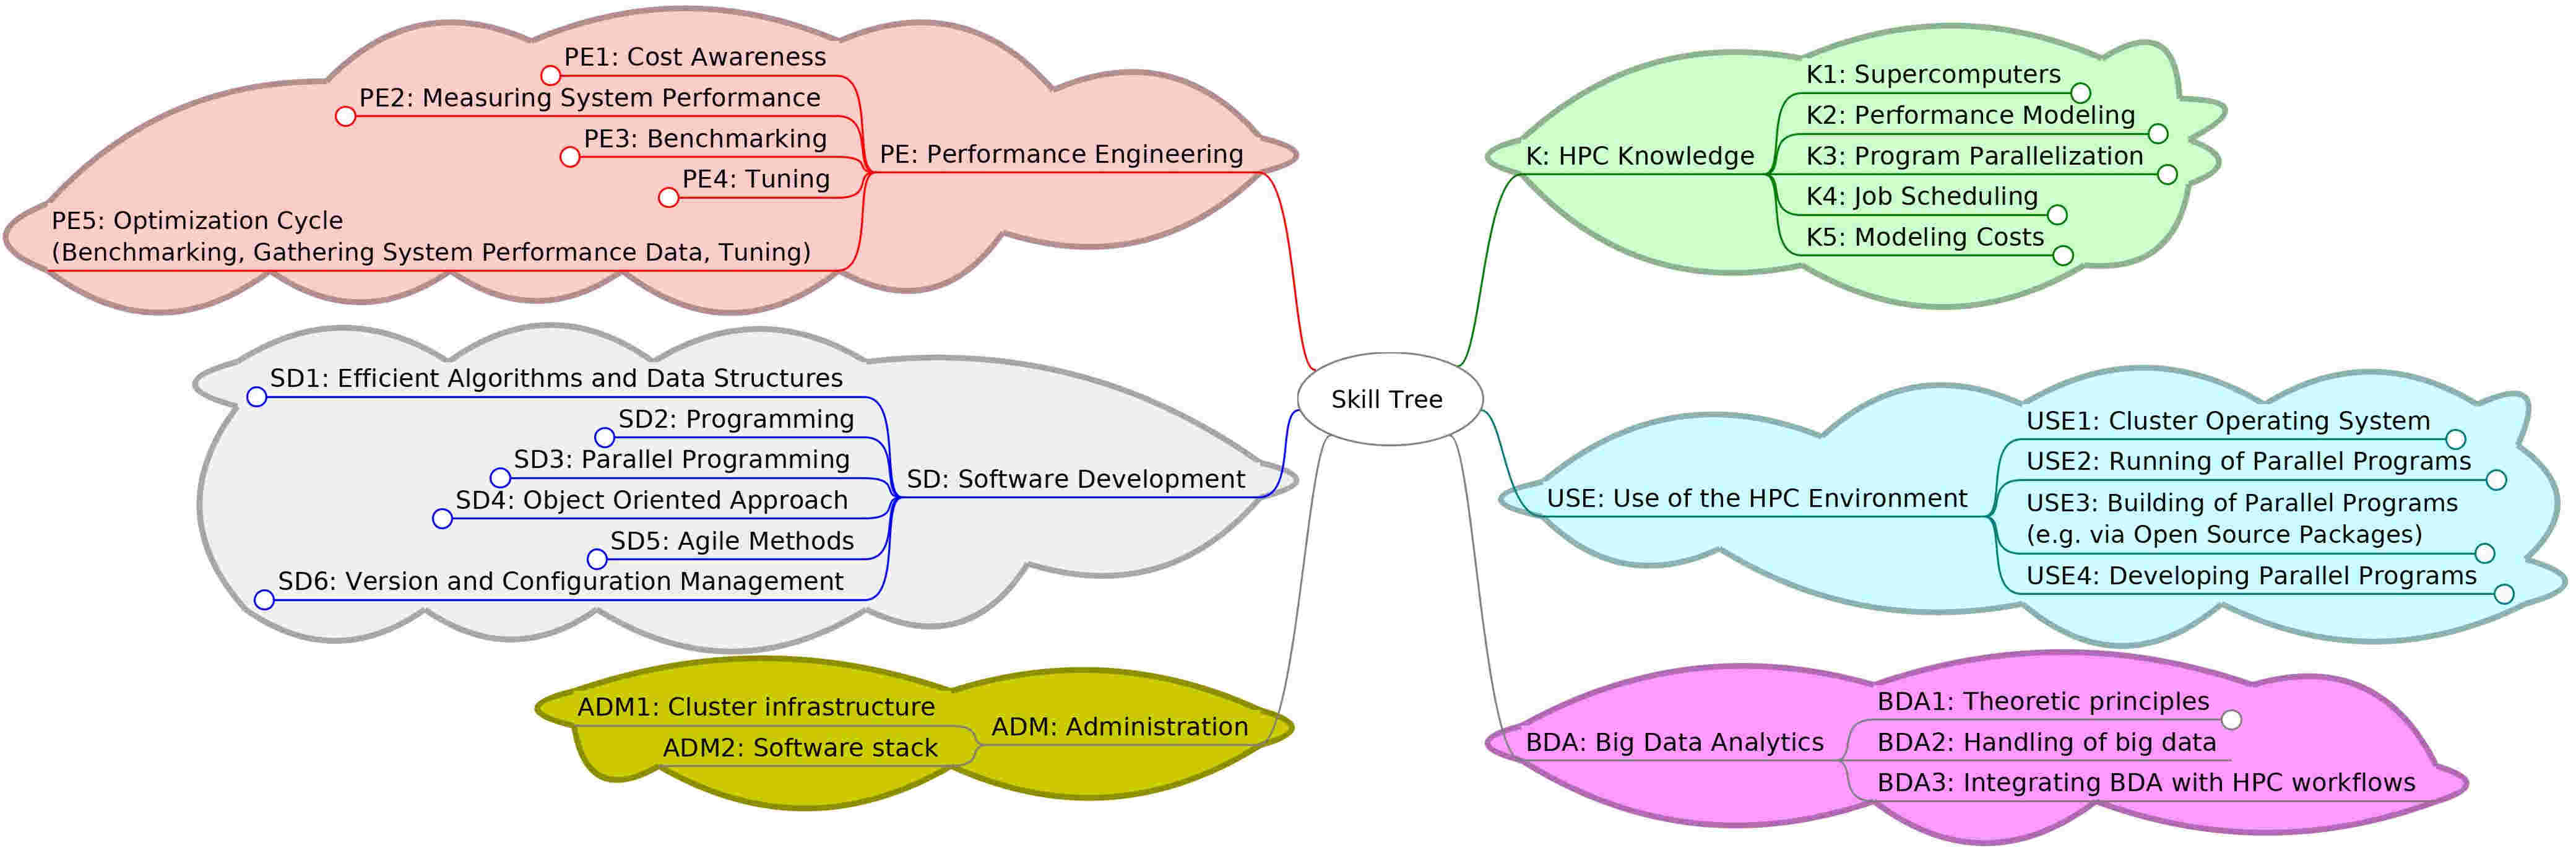
\includegraphics[width=\textwidth]{skill-tree}
		\vspace*{-2em}
		\caption{Top-levels of the skill tree (Initial ADM and BDA branches)}
	\end{figure}
\end{frame}

\begin{frame}{Example High-Level Skill (Excerpt)}
\begin{itemize}
\item Name: Command Line Interface
\item Id: USE1.1-B
\item Background: {\small HPC systems are usually accessed via a Linux-based Command Line Interface (CLI) that is provided by a shell.
At its core, a shell is ...}
\item Aim:
\begin{itemize}
\item describe the key principles of a shell
\item execute basic programs to query system information and manipulate...
\end{itemize}
\end{itemize}

\begin{block}{Learning outcomes (these must be examinable)}
\begin{itemize}
\item Utilize the bash shell to execute individual programs with arguments
\item Describe the meaning of the exit code of a program
\item Run multiple programs after another depending on the exit code ;, \&\&, ||
\item List the set of basic programs and their tasks:
\begin{itemize}
  \item pwd
  \item ... See \url{https://www.hpc-certification.org/wiki/skill-tree/use/1/1/b}
\end{itemize}
\end{itemize}
\end{block}
\end{frame}

\begin{frame}{Classification of HPC Competences}
	\begin{itemize}
		\item Granularity of skill descriptions
		\begin{itemize}
			\item Too fine $\Rightarrow$ content of a skill is predefined at leaf level
			\item Too coarse $\Rightarrow$ no help for structuring the material
			\item Guiding principle: leaf node should be coverable in 1-4 hour lecture/workshop
		\end{itemize}


    \item Organization of HPC skills
    \begin{itemize}
      \item Skills are typically depending on sub-skills $\Rightarrow$ tree structure
      \item References to skills are possible; still skills are building blocks for various tasks
      \item One skill can have multiple instances for different skill levels (basic, ..., expert)
    \end{itemize}


    \item Verification of skill tree and certification approach
      \begin{itemize}
        \item Feedback by the HPC community/practitioners justify the approaches
      \end{itemize}
	\end{itemize}
\end{frame}



\begin{frame}{Further Considerations}
	\begin{itemize}
		\item Certificate definition
		\begin{itemize}
			\item Bundles a set of useful skills together %(e.g. "Getting startet with HPC Clusters")
			\item A users' HPC qualification is certified by successful exams
      \item Testing a single (fine-grained) skill may be too easy with a cheat sheet
		\end{itemize}
		\item Separation of \textbf{skill}, \textbf{certificates} and \textbf{content provider}
		\begin{itemize}
			\item Similar to the concept of a high school graduation exam %("Zentralabitur")
			\item Learning material can be provided by different institutions
			\item Teachers can put badges on material: this "trains skills X, Y, Z"
		\end{itemize}
  	\item External information can be linked to the skills providing different \textbf{views}
		\begin{itemize}
			\item Suitability for a user role (Tester, Builder, Developer)
			\item Suitability for a scientific domain (Chemistry, Physics, ...)
			\item View: purpose-specific representation / coloring / content
				\begin{itemize}
				\item Groups/institutions can derive a new skill tree with their own emphasis
				\item  What should people know to effectively work in your environment?
				\end{itemize}
		\end{itemize}
	\end{itemize}
\end{frame}


\begin{frame}{Status / Previous Activities}

\begin{columns}
\column{0.8\textwidth}
	\begin{itemize}
	\item The development version of the Competence Standard is online
	\item Released technical representations of the HPC skills
    \begin{itemize}
      \item Markdown (embedded in a Wiki)
    \end{itemize}
	\item Released JavaScript for visualization of skill tree \hrefb{https://www.hpc-certification.org/skills/}{(demo)}
		\begin{itemize}
			\item Enables views: adjustable/embedable in your webpage
		\end{itemize}
	\item Developed prototype for exam process and framework
  \item Developed various processes
	\item Designed seal of endorsement
	\item Engaged with various stakeholders (e.g., SIGHPC Edu)
	\item Conducted survey to verify the skill tree (more to come!)
\end{itemize}

\column{0.2\textwidth}
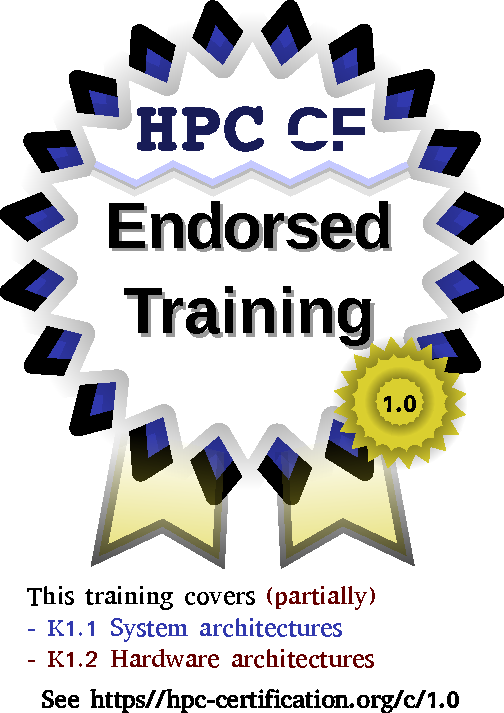
\includegraphics[width=\textwidth]{certified.pdf}
\end{columns}

\medskip

\textit{All our developments are under open licenses (except the exam questions)}
\end{frame}


\begin{frame}{Wiki for Skills}
  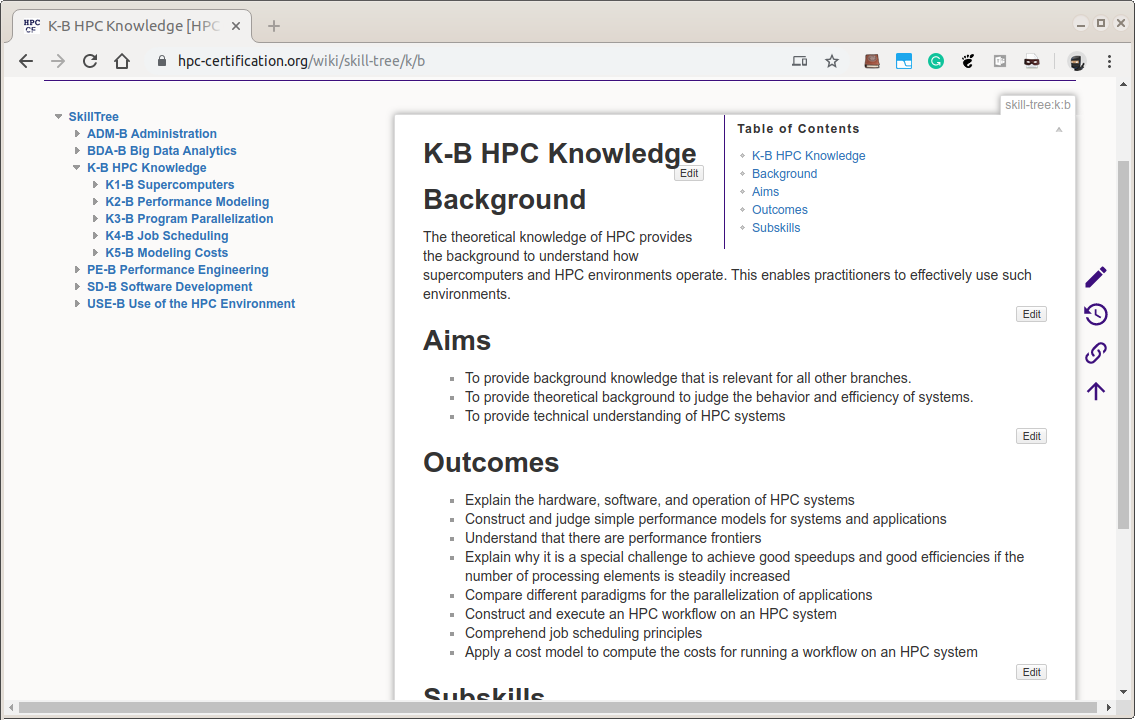
\includegraphics[width=0.8\textwidth]{www}
\end{frame}


\begin{frame}{Contribution to the Skill-Tree High-Level Editing}

  \begin{block}{How can members contribute?}
  \begin{itemize}
    \item Webpage with Markdown version controlled in Git
      \begin{itemize}
        \item \url{https://www.hpc-certification.org/wiki/skill-tree/b}
        \item GitHub: \url{https://github.com/HPC-certification-forum/skill-tree}
        \begin{itemize}
          \item Pull requests, reviews, comments, ...
        \end{itemize}
      \end{itemize}
    \item Editing a MindMap, the structure of Skills
      \begin{itemize}
        \item Synchronized with the skill tree in Git
        \item Uses the OpenSource tool Freemind
      \end{itemize}
    \item Discussion on our \href{https://join.slack.com/t/hpc-certification/shared_invite/enQtMzUwNzU3NzM2MTkzLTAzZWM3NDg0N2I2ZmQwOWI5ZGUwNjNlNDgzM2RmOTM3ZWRjNjIxYTc5NzUxYTJhNmRlNmM5YmE1NDY3YzkzYzA}{Slack}
    \item Details in our videos on YouTube:
    \url{https://www.youtube.com/playlist?list=PL4b682pSp7MQbdhhvwisrPo7PjYya26_g}
  \end{itemize}
  \end{block}
\end{frame}



\section{Certification Process}
\sectionIntroHidden

\begin{frame}{Certification: Assessment Prototype}
		\begin{itemize}
			\item[\color{readingRed}{1.}] User takes multiple-choice test online (any time!)
			\begin{itemize}
				\item A combination of JavaScript and a web service
				\item System selects number of questions randomly from a pool
					\begin{itemize}
						\item The questions are managed with rigorous license agreement
					\end{itemize}
				\item System draws 4-5 responses from 10 possible responses (some randomized)
			\end{itemize}
			\item[\color{readingRed}{2.}] Choices are submitted to the web server
			\item[\color{readingRed}{3.}] \textit{Approval} of the result
			\item[\color{readingRed}{4.}] Automatic creation of certificate and returned by email
			\begin{itemize}
							\item Permanent computer-verifiable proof that skill is created
							\begin{itemize}
								\item Return a text version with GPG signature
								\item Return a link that can be verified on hpc-certification.org
							\end{itemize}
			\end{itemize}
			\item Privacy: minimize information stored on servers, keep some for statistics
			\item Includes some measure to prevent cheating and brute forcing (e.g., delay)
		\end{itemize}
\end{frame}

\begin{frame}[fragile]{Certification: Certificate}
\begin{columns}
	\column{0.6\textwidth}
	\begin{block}{Text representation}

		\scriptsize
		\begin{verbatim}
-----BEGIN PGP SIGNED MESSAGE-----
Hash: SHA512
HPC Certification Forum Certificate
This text confirms that "Jane Doe" has
successfully obtained the certificate
"HPC driving license" (id: 1) at 02/2019.
Verification URL: https://hpc-certification.org/[...]
-----BEGIN PGP SIGNATURE-----
[...]
-----END PGP SIGNATURE-----
		\end{verbatim}
	\end{block}

\column{0.4\textwidth}
	\begin{block}{Certificate}
		\medskip
		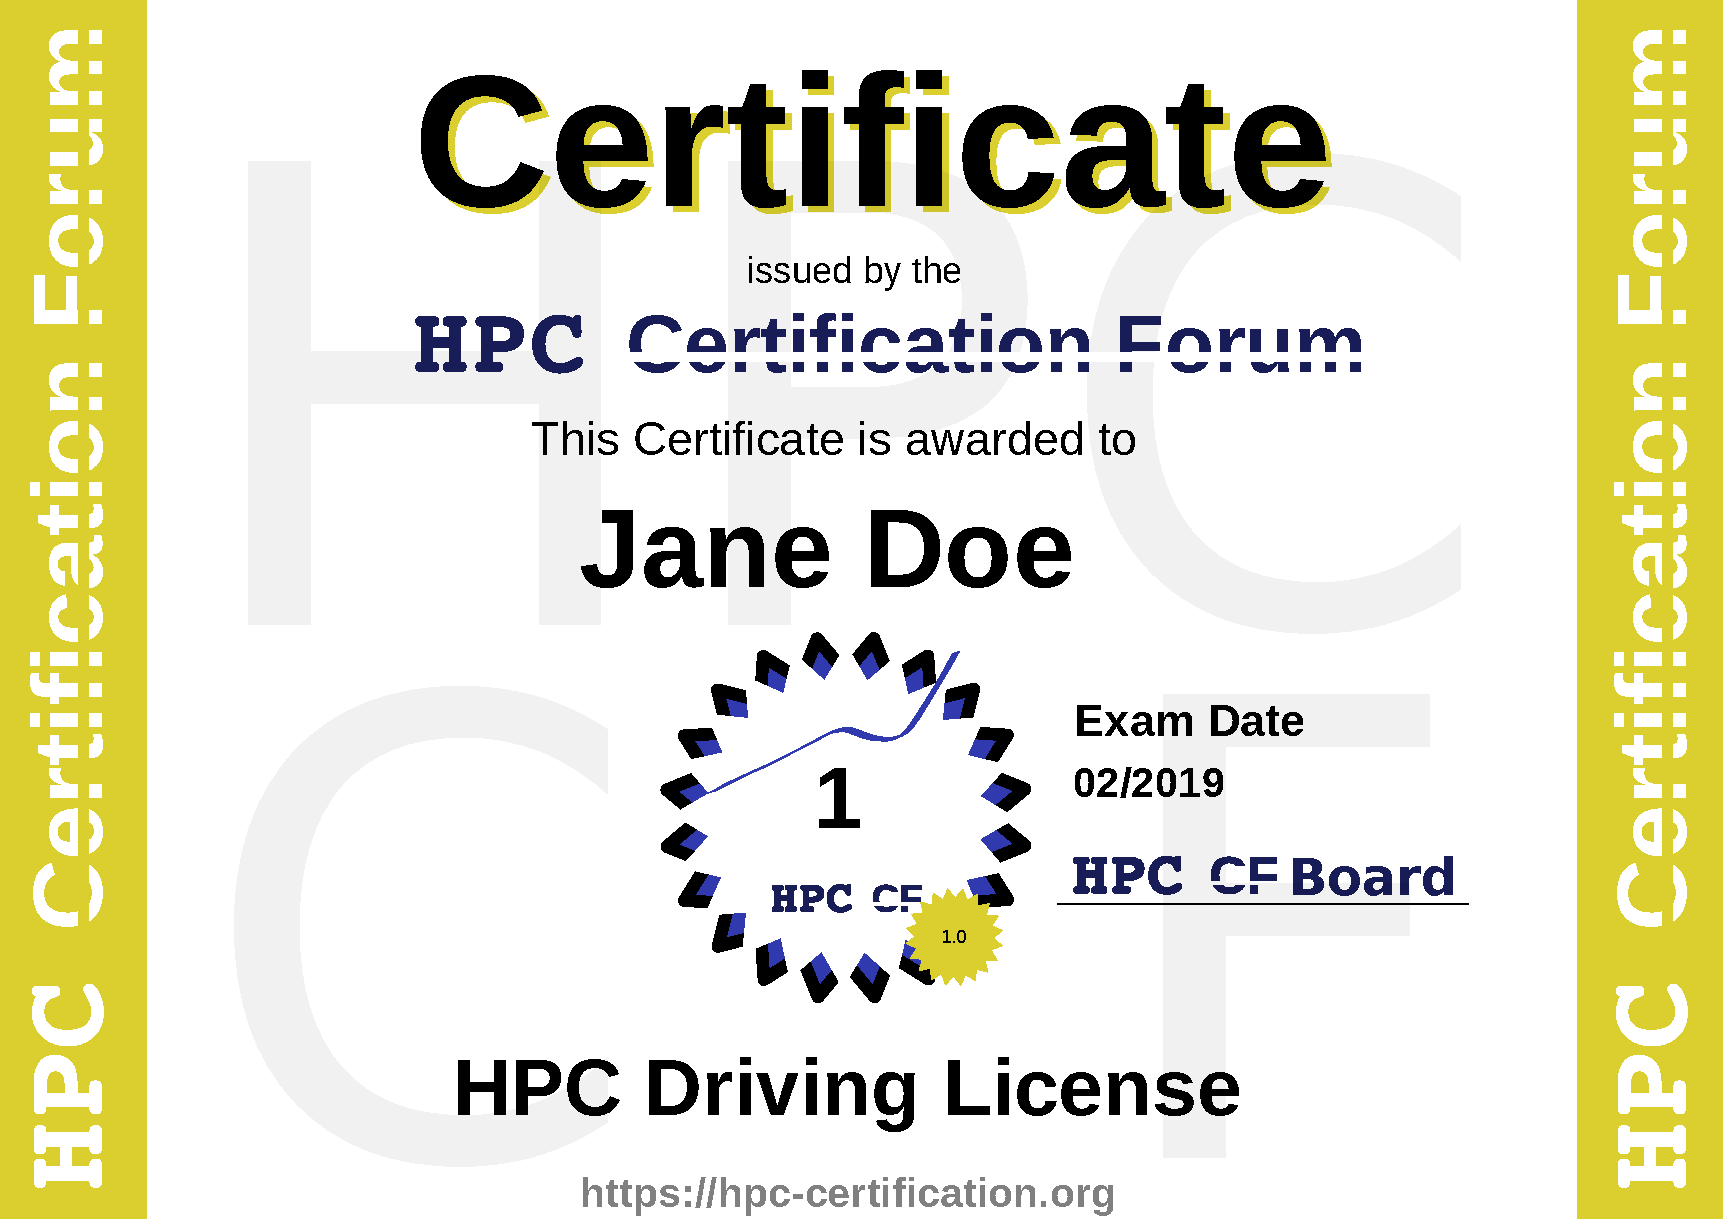
\includegraphics[width=\textwidth]{jane-doe}
	\end{block}
\end{columns}
\end{frame}

\begin{frame}{Relevance for OSS}
  \begin{itemize}
    \item HPC skills require Linux knowledge
    \item Maybe the concepts for HPC-CF is relevant generally to practitioners?
    \item Open, free, and fine-grained certification would be great to have for Linux!
  \end{itemize}

  \begin{block}{New: Experts Adopting Skills}
  \begin{itemize}
  \item Enable experts to curate skills that are in their field of expertise
  \item Similar to code maintainer
  \end{itemize}
  \end{block}
\end{frame}



\section{Conclusions}
\sectionIntroHidden

\begin{frame}{Outlook and Expected Benefits}
	\begin{block}{HPC practitioners}
		\vspace*{-0.2cm}
	\begin{itemize}
	\item Increase motivation to participate as the certificates are recognized in a CV
	\item Validate knowledge via tests
	\item Browse relevant competences
	\item Identify recommended and required skills related to certain tasks
	\item Understand and compare teaching offers across sites
	\end{itemize}
	\end{block}
	\vspace*{-0.3cm}
	\begin{block}{Data centers}
		\vspace*{-0.2cm}
	\begin{itemize}
	\item Increase sharing of teaching materials
	\item Simplifies documentation of taught skills
	\item Identify missing teaching activities
	\item Tailor skill-representation specifically to users
	\item Correlate lack of skills with efficient use
	\end{itemize}
	\end{block}
\end{frame}



\begin{frame}{Summary}

	\begin{block}{HPC Certification Program}
		\begin{itemize}
			\item Effort to standardize representation/certification of relevant HPC skills
      \begin{itemize}
        \item Hierarchical definition of skills for practitioners
        \item Building blocks that can be cherry-picked for different tasks
				\item It's goal is \textbf{NOT} to provide content or a linear curriculum
      \end{itemize}
			\item Perspective for data centers
				\begin{itemize}
					\item Use statistics and machine learning to direct users to right skills
					\item Make certain skills a mandatory requirement?
				\end{itemize}
			\item Customizable representation and navigation for data centers/domains
      \begin{itemize}
        \item Interactive viewer to browse skills and related content
				\item We will use the viewer to link good content to the skills, too!
      \end{itemize}
      \item Visit us and join our Slack/mailing lists: \url{https://hpc-certification.org}
		\end{itemize}
	\end{block}
\end{frame}




\end{document}
